\documentclass[11pt]{standalone}
\usepackage{amssymb}
\usepackage{amsmath}
\usepackage[no-math]{fontspec}
\usepackage{unicode-math}
\usepackage{libertinus}
\usepackage{pgf,xcolor}
\usepackage{tikz}
\usetikzlibrary{arrows.meta, backgrounds}
\usepackage{pgfplots}
\pgfplotsset{compat=newest}

\definecolor{my_darkgray}{HTML}{484949}
\definecolor{my_lightgray}{HTML}{F3F4F4}
\definecolor{my_darkblue}{HTML}{005A94}
\definecolor{my_lightblue}{HTML}{CCDEE9}
\definecolor{my_yellow}{HTML}{FFEC7F}
\definecolor{my_red}{HTML}{E60000}
\definecolor{my_orange}{HTML}{E87846}

%% Fourier coefficients of the asymmetric rectangular signal
%%   f(t) = 2  on [0, T/2),  f(t) = -1 on [T/2, T),  T = 40 ms
%%   a_0 = 1  (mean value a_0/2 = 0.5)
%%   a_n = 0  for all n >= 1
%%   b_n = 6/(n*pi)  for odd n,  b_n = 0  for even n
%%
%% Partial sums (t in ms, omega_0*t = pi*t/20):
%%   S_1 = 0.5 + (6/pi)*sin(pi*x/20)
%%   S_3 = S_1  + (6/(3*pi))*sin(3*pi*x/20)
%%   S_7 = S_3  + (6/(5*pi))*sin(5*pi*x/20) + (6/(7*pi))*sin(7*pi*x/20)
%%
%% Step function (const plot, two periods from t = -40 to 80 ms):
%%   [-40,-20): f = 2,  [-20,0): f = -1,  [0,20): f = 2,
%%   [20,40): f = -1,  [40,60): f = 2,  [60,80): f = -1

\begin{document}
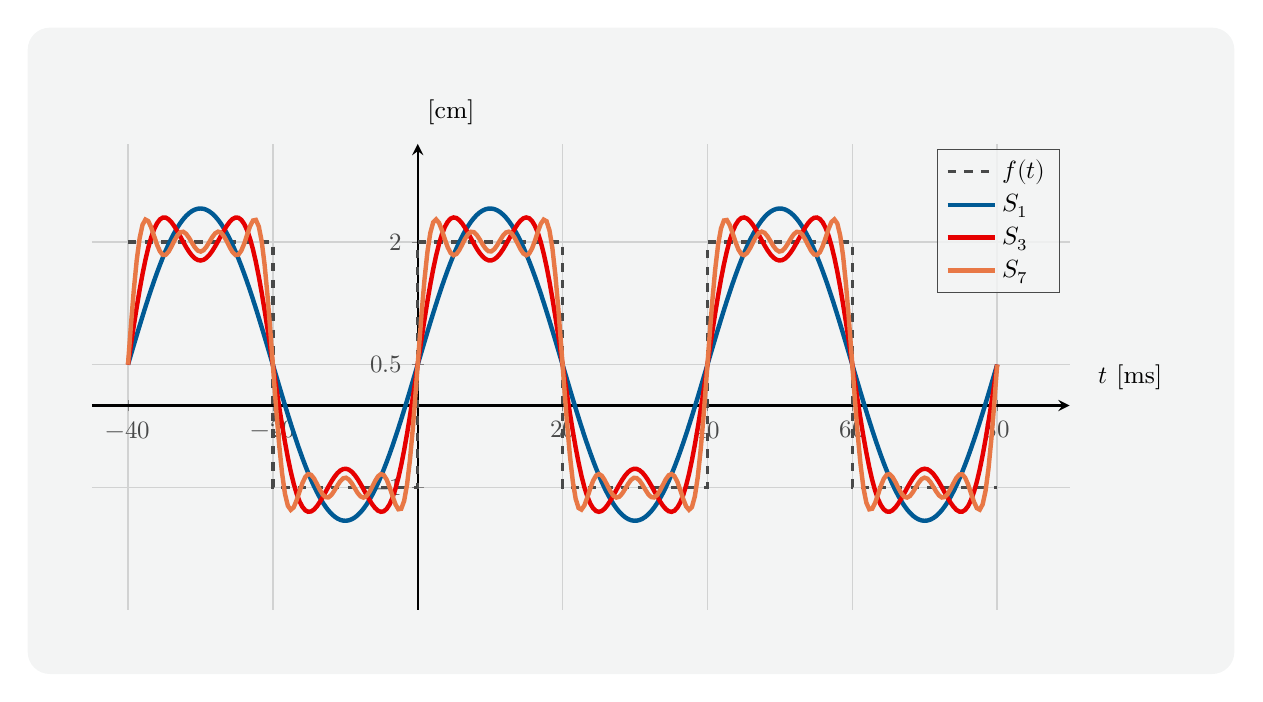
\begin{tikzpicture}[
    show background rectangle,
    background rectangle/.style={fill=my_lightgray, rounded corners=8pt},
    inner frame sep=0.8cm
]

\begin{axis}[
    axis lines = center,
    xlabel = {$t$ [ms]},
    ylabel = {[cm]},
    xlabel style={at={(axis description cs:1.02,0.5)}, anchor=west, font=\small},
    ylabel style={at={(ticklabel* cs:1.02)}, anchor=south west, font=\small},
    xmin = -45,
    xmax = 90,
    ymin = -2.5,
    ymax = 3.2,
    xtick = {-40, -20, 0, 20, 40, 60, 80},
    ytick = {-1, 0, 0.5, 2},
    yticklabels = {$-1$, $0$, $0.5$, $2$},
    axis line style = {thick},
    grid = both,
    grid style = {draw=my_lightgray!60!white, line width=0.4pt},
    major grid style = {draw=my_lightgray!80!my_darkgray, line width=0.5pt},
    tick label style = {font=\small, color=my_darkgray},
    width = 14cm,
    height = 7.5cm,
    % axis equal not used: time axis (ms) vs displacement (cm) have different units
    legend style = {
        at={(0.99, 0.99)},
        anchor=north east,
        font=\small,
        fill=my_lightgray,
        draw=my_darkgray,
        fill opacity=0.85,
        text opacity=1,
    },
    legend cell align=left,
]

%% --- Rectangular target signal f(t) ---
\addplot[
    const plot,
    draw = my_darkgray,
    dashed,
    line width = 1.2pt,
    no marks,
]
coordinates {(-40,2) (-20,-1) (0,2) (20,-1) (40,2) (60,-1) (80,-1)};
\addlegendentry{$f(t)$}

%% --- S_1 ---
\addplot[
    draw = my_darkblue,
    ultra thick,
    samples = 300,
    domain = -40:80,
]{
    0.5
    + (6/pi)*sin(deg(pi*x/20))
};
\addlegendentry{$S_1$}

%% --- S_3 ---
\addplot[
    draw = my_red,
    ultra thick,
    samples = 300,
    domain = -40:80,
]{
    0.5
    + (6/pi)*sin(deg(pi*x/20))
    + (6/(3*pi))*sin(deg(3*pi*x/20))
};
\addlegendentry{$S_3$}

%% --- S_7 ---
\addplot[
    draw = my_orange,
    ultra thick,
    samples = 300,
    domain = -40:80,
]{
    0.5
    + (6/pi)*sin(deg(pi*x/20))
    + (6/(3*pi))*sin(deg(3*pi*x/20))
    + (6/(5*pi))*sin(deg(5*pi*x/20))
    + (6/(7*pi))*sin(deg(7*pi*x/20))
};
\addlegendentry{$S_7$}

\end{axis}

\end{tikzpicture}
\end{document}
